%---------- Inleiding ---------------------------------------------------------

% TODO: Is dit voorstel gebaseerd op een paper van Research Methods die je
% vorig jaar hebt ingediend? Heb je daarbij eventueel samengewerkt met een
% andere student?
% Zo ja, haal dan de tekst hieronder uit commentaar en pas aan.

%\paragraph{Opmerking}

% Dit voorstel is gebaseerd op het onderzoeksvoorstel dat werd geschreven in het
% kader van het vak Research Methods dat ik (vorig/dit) academiejaar heb
% uitgewerkt (met medesturent VOORNAAM NAAM als mede-auteur).
% 
\newcommand{\figref}[1]{(Zie \hyperref[#1]{figuur: \ref{#1}})}

\section{Inleiding}%
\label{sec:inleiding}

In de hedendaagse samenleving is er een groeiende behoefte aan technologieën die de communicatie tussen doven en horenden vergemakkelijken. Een veelbelovende ontwikkeling is de real-time vertaling van Vlaamse Gebarentaal (VGT) naar tekst met behulp van kunstmatige intelligentie (AI) en computer vision. VGT, de taal van de Vlaamse dovengemeenschap, is een erkende taal met regionale variaties, wat de vertaling bemoeilijkt \autocite{vanmeerbergen2000simultane}.

Dit onderzoek richt zich op de inzet van AI-technologieën voor het herkennen en vertalen van VGT-gebaren naar tekst om de communicatie en inclusie van de dove gemeenschap te bevorderen. De centrale vraag is: "Hoe kunnen AI-technologieën worden ingezet voor de real-time vertaling van Vlaamse Gebarentaal naar tekst?" We onderzoeken de volgende deelvragen:

\begin{enumerate} 
  \item Welke AI-technologieën zijn beschikbaar voor gebarentaalherkenning en hoe effectief zijn deze al? 
  \item Hoe kunnen we verder bouwen op al bestaande gebarentaal herkenning? 
  \item Welke uitdagingen en beperkingen zijn er bij het ontwikkelen van een vertalingssysteem voor VGT? 
  \item Hoe kan zo'n systeem de communicatie en inclusie van de dove gemeenschap verbeteren? 
\end{enumerate}

De structuur van VGT is complex, met variaties in handvorm, beweging en gezichtsuitdrukkingen \autocite{469340}. Geavanceerde algoritmen zoals deep learning en convolutionele neurale netwerken (CNN) zijn veelbelovend voor gebarentaalherkenning \autocite{10.52756/ijerr.2023.v34spl.004}\autocite{10.17485/ijst/v16i45.2583}. Met camera's op smartphones kunnen systemen worden ontwikkeld die gebaren in real-time omzetten naar tekst.

Deze technologische vooruitgang kan de toegankelijkheid en inclusie van de dove gemeenschap aanzienlijk verbeteren. Dit document onderzoekt de huidige stand van zaken van AI-gestuurde VGT-herkenning, en de toepassingen en uitdagingen van dergelijke systemen.
\section{Literatuurstudie}%
\label{sec:literatuurstudie}

\subsection{Vlaamse Gebarentaal}
\label{subsec:vgt}

Het Vlaamse Gebarentaal (VGT) is een visuele taal die wordt gebruikt door de Vlaamse dovengemeenschap. 
Het is een volwaardige taal met een eigen grammatica en lexicon, die verschilt van gesproken talen zoals Nederlands en Frans. 
VGT maakt gebruik van handgebaren, gezichtsuitdrukkingen en lichaamstaal om betekenis over te brengen. 
Het is belangrijk op te merken dat VGT, net als gesproken talen, regionale variaties kent, wat de complexiteit van de vertaling vergroot \autocite{469340}.
Dit betekent dus dat het model dat wordt ontwikkeld rekening moet houden met deze regionale variaties.
Er zijn in totaal 5 variaties op het VGT, deze zijn ook regionaal gebonden\autocite{469340}.
De variaties zijn: West-Vlaanderen, OostVlaanderen, Antwerpen, Limburg en Vlaams-Brabant.
Het kan echter ook zijn dat bepaalde gebaren in de ene regio hetzelfde zijn als in een andere regio.
Maar de variatie in deze regionale gebaren is niet direct significant.
Uit studies van \textcite{469340} blijkt dat 72.3\% van de gebaren in de verschillende regio's identieke verwante of verwante gebaren tonen.
Hierbij blijkt zelf de antwerpse variant de centraalste variant te zijn\autocite{469340}.
Maar het is wel belangrijk om hier rekening mee te houden.


\subsection{Data-acquisitie}
\label{subsec:data-acquisitie}

Het verzamelen van data is een cruciale stap in het ontwikkelen van een AI-model voor VGT-herkenning.
Er zijn verschillende manieren om data te verzamelen, waaronder het gebruik van bestaande datasets en het opnemen van nieuwe datasets met behulp van camera's.
Een van de meest gebruikte datasets voor VGT-herkenning is de VGT-dataset van de Universiteit van Gent\autocite{VGT_Signbank}.
Voor deze dataset moet toegang aangevraagd worden aan de Universiteit van Gent.
Een andere optie voor deze dataset is om hun website te scrapen en zelf te labelen.
Er zijn ook andere datasets beschikbaar, zoals het VGT-corpus van de Universiteit van Leuven\textcite{Corpus_VGT}.
Deze datasets bevatten video-gesprekken van VGT-gebaren.
Er is ook een gedeelde met de gelabelde data en annotaties van de video's.
Hier zijn ze echter nog aan aan het werken en vereist speciale toegang\autocite{Over_het_Corpus_VGT}.
Een andere optie is om zelf een dataset te maken door VGT-gebaren op te nemen met behulp van een camera.
Dit kan gedaan worden door een camera te gebruiken die is aangesloten op een computer of door een smartphone te gebruiken.
Er kan getwijfeld worden over de grote van deze dataset maar onderzoek van \textcite{Coster2023} toont aan dat een van deze dataset groot genoeg is om een model te trainen met goede accuratie.
Een ander probleem dat zich kan voordoen is dat de data niet in het juiste formaat is voor een model efficient of goed te trainen\autocite{Vandeghinste2024}.


\subsection{Modeltraining}
\label{subsec:modeltraining}
Voor het model te trainen zal er gebruik gemaakt worden van deep learning.
Er zijn meerdere mogelijke manieren om modellen te trainen. 
Een van de meest gebruikte type modellen voor Gebarentaal-herkenning is het convolutionele neurale netwerk (CNN).
Dit type model is al reeds effectief gebleken in het halen van handgebaren en gezichtsuitdrukkingen in gebarentaal video's\autocite{10.17485/ijst/v16i45.2583}.
Een optie binnenin convolutionele neurale netwerken is transfer learning.
Dit is een techniek waarbij een model wordt getraind op een grote dataset en vervolgens wordt aangepast aan een specifieke of verwante taak\autocite{torrey2010transfer}.
Meestal gebruieken ze hiervoor al een bestaand model dat al getraind.
Er zijn meerdere modellen waarbij deze techniek zou toegepast kunnen worden.
Het zou kunnen op een gewoon image classification model zoals VGG16 of ResNet.
VGG16 is een model gemaakt door Visual Geometry Group van de Universiteit van Oxford.
Het is een model dat goed presteert op image classification en zou dus ook goed kunnen presteren op VGT-herkenning.
VGG16 wordt vaker gebruikt om transfer learning toe te passen.
Zoals bijvoorbeeld in \textcite{9491631} waar ze VGG16 gebruiken om borstkanker te herkennen.
Het werd zelf al gebruikt voor gebarentaalherkenning in \textcite{Abu-Jamie2022-ABUCOS-2}.
ResNet, of Residual Network, is een ander baanbrekend model dat is ontwikkeld door Kaiming He.
Net zoals VGG16 is ResNet een model dat goed presteert op image classification en zou dus ook goed kunnen presteren op VGT-herkenning.
Het werd ook al eerder gebruikt voor gebarentaalherkenning in \textcite{Wang2022}.
Het zou ook kunnen om transfer learning toe te passen op een model dat zelf al gebarentaal herkent.



% Voor literatuurverwijzingen zijn er twee belangrijke commando's:
% \autocite{KEY} => (Auteur, jaartal) Gebruik dit als de naam van de auteur
%   geen onderdeel is van de zin.
% \textcite{KEY} => Auteur (jaartal)  Gebruik dit als de auteursnaam wel een
%   functie heeft in de zin (bv. ``Uit onderzoek door Doll & Hill (1954) bleek
%   ...'')

%---------- Methodologie ------------------------------------------------------
\section{Methodologie}%
\label{sec:methodologie}
\subsection{Fase 1: Data-acquisitie}
In de eerste en meest cruciale fase van het onderzoek zal de benodigde data worden verzameld.
Voor het verzamelen van de data zal gebruik worden gemaakt van verschillende bronnen.
Deze bronnen zullen bestaan uit bestaande datasets, zoals de VGT-dataset van de Universiteit van Gent.
Daarnaast zullen er ook nieuwe datasets worden gecreëerd door middel van het opnemen van VGT-gebaren met behulp van een camera.
Deze datasets zullen worden gebruikt om het model te trainen en te valideren.
Voor deze fase een periode van 2 weken duren\figref{fig:gantt_tijd}.
\subsection{Fase 2: Preprocessing}
Voor het Preprocessen van de data wordt er weer een werktijd van 2 weken voorzien\figref{fig:gantt_tijd}.
Hier zullen de datasets worden geanalyseerd en gezuiverd.
De datasets zullen samengevoegd worden tot één dataset en worden opgedeeld in een trainingsset en een testset.
Het zal ook alle data juist labelen als dit nog niet correct is gebeurd.
\subsection{Fase 3: Modeltraining}
In de derde fase van het onderzoek zal het model worden getraind.
Dit zal de meeste tijd innemen van het onderzoek, namelijk 4 weken\figref{fig:gantt_tijd}.
Er zal een deep learning model worden gezocht dat al in staat is om gebarentaal te herkennen en om te zetten in tekst.
Hierbij zal er dus gebruik gemaakt worden van transfer learning.
Het startmodel zal gekozen worden op basis van de literatuurstudie.
De modellen trainen zelf zal 3 weken duren en de laatste week zal dienen om de modellen te testen en te vergelijken\figref{fig:gantt_tijd}.
\subsection{Fase 4: Model optimalisatie}
In de vierde fase van het onderzoek zal het getrainde model worden aangepast zodat het efficienter zal werken.
Deze fase zal 4 weken duren\figref{fig:gantt_tijd}.
Hier zal prunning en quantization worden toegepast om het model te optimaliseren voor mogelijk real-time gebruik.
\subsection{Fase 5: Evaluatie \& Validatie}
In de laatste fase van het onderzoek zal het model worden geëvalueerd en gevalideerd.
Deze fase zal 2 weken duren\figref{fig:gantt_tijd}.
Het model zal worden getest op een nieuwe dataset en de resultaten zullen worden geanalyseerd.
Moesten er nog enige fouten zijn in het model zullen deze worden aangepast en zal het model opnieuw worden getest.

\begin{figure}[h!]
  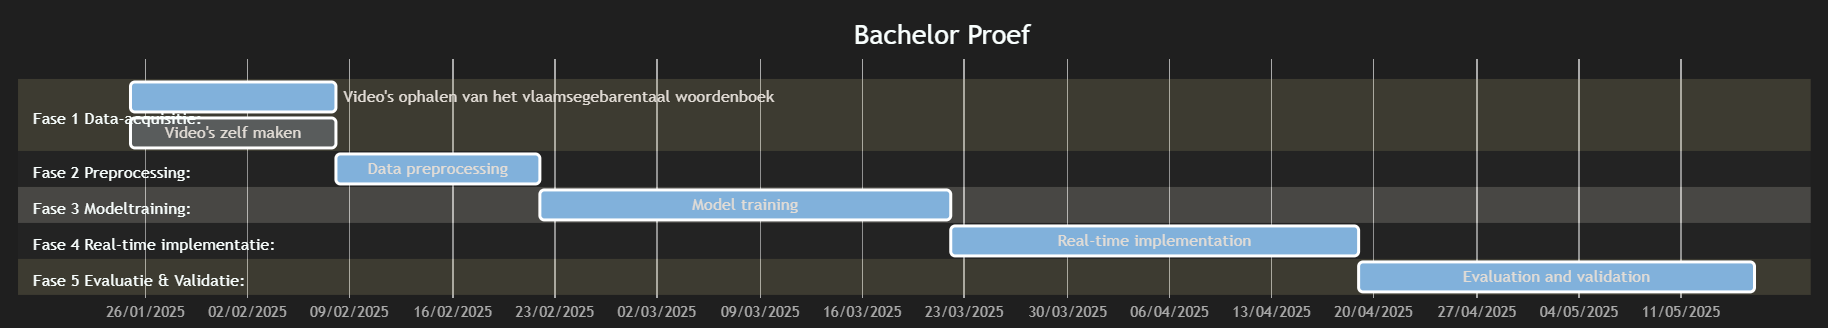
\includegraphics[width=0.5\textwidth]{../graphics/gantt_tijd.png}
  \caption{tijdlijn van het onderzoek}
  \label{fig:gantt_tijd}
\end{figure}
%---------- Verwachte resultaten ----------------------------------------------

\section{Verwacht resultaat, conclusie}%
\label{sec:verwachte_resultaten}
\subsection{Verwachte resultaten} Allereerst verwachten we dat het ontwikkelde AI-model in staat zal zijn om Vlaamse Gebarentaal (VGT) gebaren nauwkeurig te herkennen en om te zetten in tekst. Door gebruik te maken van geavanceerde deep learning technieken zoals convolutionele neurale netwerken (CNN) en transfer learning, zouden de modellen een hoge mate van nauwkeurigheid moeten behalen, zelfs bij de complexiteit van VGT's regionale variaties.

Daarnaast zal de real-time implementatie van het model, geoptimaliseerd door technieken zoals pruning en quantization, naar verwachting effectief functioneren op smartphones en andere draagbare apparaten. Dit zou betekenen dat gebruikers in staat zullen zijn om direct gebaren te vertalen naar tekst zonder merkbare vertraging, wat de bruikbaarheid en toegankelijkheid van het systeem aanzienlijk zal vergroten.

We verwachten ook dat de evaluatie van het model positieve resultaten zal laten zien wat betreft de generaliseerbaarheid en robuustheid van het model. Dit betekent dat het model niet alleen goed zal presteren op de trainingsdata, maar ook effectief zal zijn op nieuwe, ongeziene data. Hierdoor kan het systeem breed toegepast worden, onafhankelijk van de specifieke dataset waarop het getraind is.

\subsection{Conclusie} In conclusie zal dit onderzoek aantonen dat AI-gestuurde VGT-herkenning een haalbare en waardevolle technologie is die de communicatie tussen doven en horenden kan verbeteren. De resultaten zullen de potentie van deep learning en computer vision benadrukken in het herkennen van complexe gebarentaal en het omzetten ervan in tekst, wat een belangrijke stap voorwaarts is in het bevorderen van inclusiviteit en toegankelijkheid voor de dove gemeenschap.

Bovendien zal het onderzoek bijdragen aan de wetenschappelijke kennis over het gebruik van AI in gebarentaalherkenning, en een basis vormen voor toekomstige studies en toepassingen in dit veld. De bevindingen kunnen ook implicaties hebben voor de ontwikkeling van vergelijkbare systemen voor andere gebarentalen wereldwijd.

Tot slot hopen we dat dit werk zal dienen als een inspiratie voor verdere innovatie in assistieve technologieën, en dat het de aandacht zal vestigen op de noodzaak van dergelijke oplossingen om de communicatiekloof tussen doven en horenden te overbruggen.